\documentclass[12pt]{article}
\usepackage{graphicx}
\usepackage{hyperref}
\usepackage{subcaption}
\usepackage{amsmath}
\usepackage{geometry}
\usepackage{float} % Include the float package
\geometry{a4paper}

\title{Comprehensive Analysis Report of the WhatsApp Group: Kissan Express}
\author{Muhammad Saad}
\date{\today}

\begin{document}

\maketitle

\section{Introduction}
This report provides a comprehensive analysis of the WhatsApp group ``Kissan Express," focusing on the content shared, user interactions, and group dynamics. The analysis aims to identify the main themes, user engagement patterns, and the relevance of the content to the group's primary purpose. By examining the messages, media, and user insights, this report offers valuable insights into the group's communication dynamics and content preferences.

\section{Data Analysis}
\subsection{Marketing Posts}
Several members use the platform to promote various services, products, or content related to agriculture. These marketing efforts range from personal introductions with professional credentials to explicit invitations to join specific platforms or groups. Below are examples of such marketing posts:

\begin{itemize}
  \item \textbf{Message 21:} A self-introduction by a media professional aiming to attract followers interested in agricultural matters.
  \item \textbf{Message 27 \& 68:} Promotes a video on wheat preservation, encouraging viewers to follow and share the content.
  \item \textbf{Message 103:} An invitation to join an external crypto platform with a referral incentive, showcasing a direct marketing approach.
  \item \textbf{Message 105:} Directly promotes a Crypto WhatsApp group, potentially to share more targeted marketing or informational content.
  \item \textbf{Message 129:} Advertises rice ready for export with detailed contact information, targeting potential buyers directly.
\end{itemize}

\subsection{Group Invitations}
The group contains only 2 invite links. One to a personal channel and the other to a crypto group. Both are irrelevant. However, there are 28 links to facebook, 8 links to youtube, and 5 links to tiktok. Only 30-40\% of the links are related to agriculture and farming.
\begin{figure}[H]
\centering
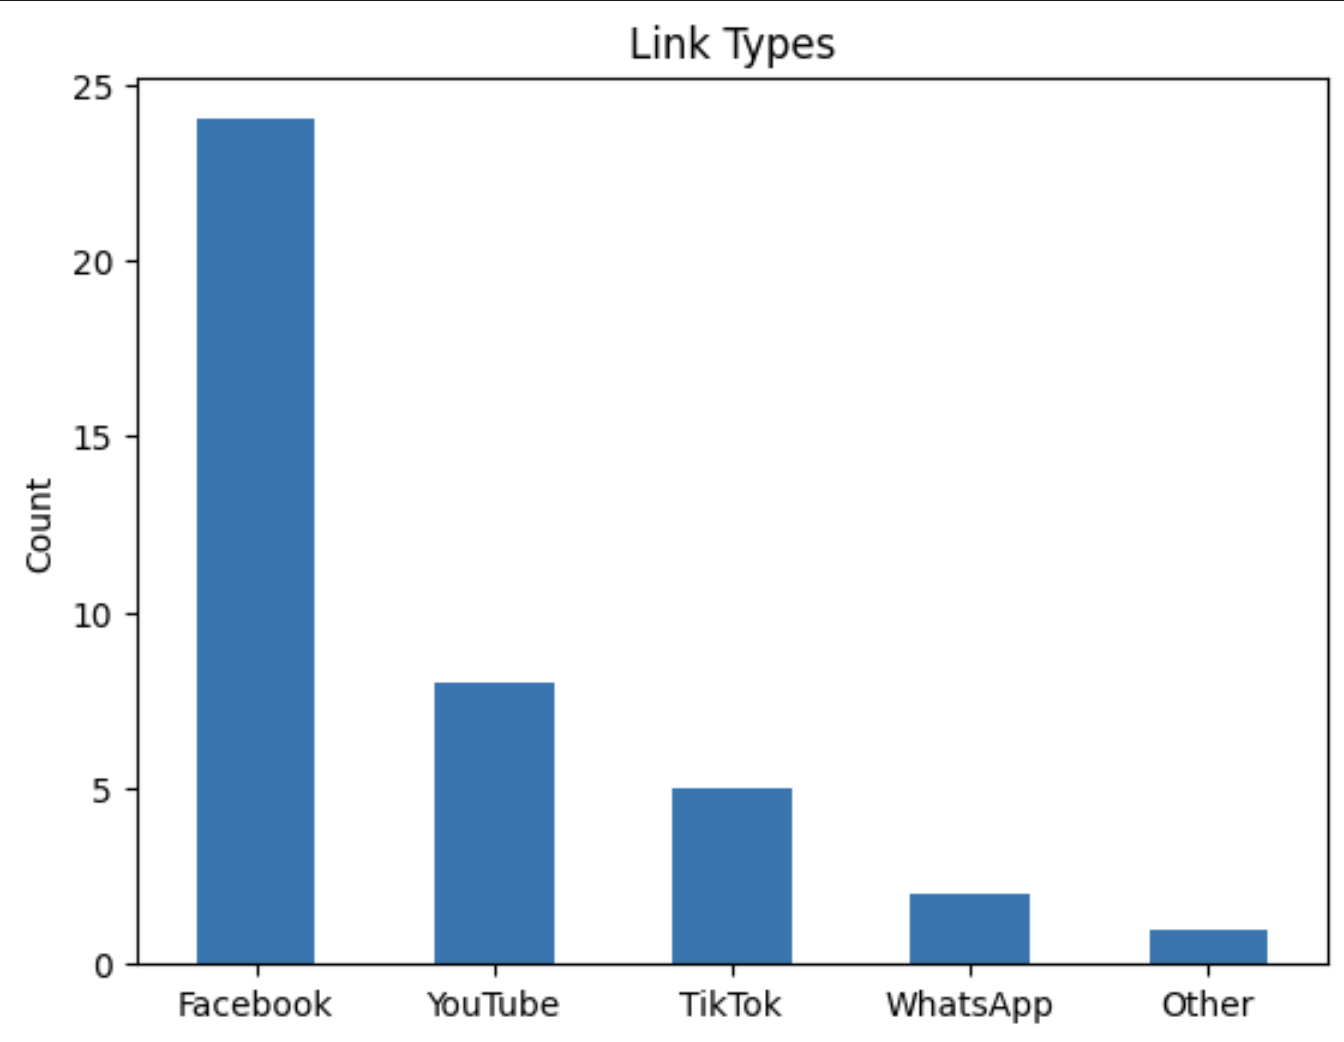
\includegraphics[width=0.8\textwidth]{img/group_invitations.png}
\caption{Group Invitations Analysis}
\end{figure}

\subsection{Response Posts}
Users do not usually interact with the other posts in the group. Replies are usually done if the user missed something in the earlier message.  \textbf{Likes} and \textbf{emojis} are the most common form of response. In general, the group does not contain any interactive discussions.



\subsection{Useful Content \& Irrelevant Content}
Detailed analysis is provided in section 3.1.

\section{Medium Analysis}
\subsection{Text Messages}

\subsubsection{Religious Messages}
These messages often contain prayers, references to religious texts, or general spiritual sentiments. Examples include:
\begin{itemize}
  \item Message 12: ``Ya Allah madad".
  \item Message 17: References a Hadith about prayer practices.
  \item Message 75: A Hadith about feeding people and greeting everyone.
  \item Message 86: A prayer for beneficial rain.
  \item Message 122: A Hadith regarding killing a chameleon.
\end{itemize}

\subsubsection{Political Messages}
These involve discussions about governmental actions, political figures, or national events. Examples include:
\begin{itemize}
  \item Message 6: References to the country's 65-year timeline.
  \item Message 7: Audit of military accounts under Imran Khan's administration.
  \item Message 8: Nawaz Sharif's statement denying ownership of London flats.
  \item Message 66: Criticism of national leadership.
\end{itemize}

\subsubsection{Useful Messages (Agriculture, Farming, etc.)}
These messages are directly relevant to the group's main theme, offering information about farming techniques, weather updates affecting agriculture, or agricultural products. Examples include:
\begin{itemize}
  \item \textbf{Rice Variety Inquiry (Messages 23 \& 24)}: Queries about "1847 rice," asking for information on its characteristics and quality, indicating a community interest in specific crop types and their cultivation details.
  \item \textbf{Wheat Preservation (Messages 27 \& 68)}: Repeated advice on methods to keep wheat safe, emphasizing the importance of proper storage techniques to maintain grain quality. The message encourages sharing this vital information widely within the community.
  \item \textbf{Fertilizers (Message 33)}: An image attachment related to "Nanocal/Calcium Fertilizer," offering a specific product that can enhance soil nutrition, crucial for crop health and yield.
  \item \textbf{Agricultural Guides (Messages 70-74)}: A series of PDF attachments providing detailed guides on cultivating various types of mushrooms (Button and Oyster) and other crops like tomatoes and chili peppers. These documents likely offer comprehensive techniques from planting to harvesting, which are essential for maximizing productivity.
  \item \textbf{Pest Control (Message 85)}: An image of "Rat Killer" pesticide, addressing the need for effective pest management solutions in agriculture, which is critical for protecting crops from rodent damage.
  \item \textbf{Tree Planting Guide (Message 91)}: Advice on which trees to plant and the methods for doing so, which is beneficial for agroforestry practices or diversifying farm outputs.
  \item \textbf{Production Plan (Message 106)}: A detailed 20-page document about the production plan for Mung and Mash for 2023-24, illustrating a structured approach to crop production planning which can help in achieving better yields and organized farming operations.
  \item \textbf{Fungicide Information (Message 115)}: Shares an image of "Air One Fungicide," which is pertinent for managing plant diseases, thereby ensuring the health and productivity of crops.
\end{itemize}

\subsection{Photos \& Videos}
\begin{itemize}
  \item \textbf{Religious and Cultural Content}: Images featuring religious calligraphy and symbols, often used to communicate spiritual messages or mark religious occasions, enhancing communal and spiritual solidarity.
  \item \textbf{Marketing and Business Promotion}: Advertisements for various services and products, such as cotton processing or herbal remedies, aimed at leveraging the community network for business purposes.
  \item \textbf{Personal and Motivational Messages}: Personal announcements or motivational messages that may include life events, accomplishments, or inspirational quotes to uplift and motivate the group members.
  \item \textbf{Informational and Advisory Posts}: Useful snippets of information including health advisories and agricultural tips like the use of rat poison in farming, intended to inform and assist the group members in practical aspects of their daily lives.
\end{itemize}


\subsection{Voice Notes}
The group contains only 1 voice note, which is about an accident near Kashmir and Neelum. Language is Punjabi I believe. Very hard to understand.

\section{User Insights}
\subsection{Number of Admins}
There are 9 admins in the group.

\subsection{Total Users}
The total number of users in the group is 718.

\subsection{Active Users}
There are 31 active users, who regularly contribute to the discussions. Top 20 are:
\begin{enumerate}
  \item Nadeem Bhatti Bhatti
  \item Master Falak Sher
  \item Ahmad Naseer
  \item Muhammad Usman
  \item Anwar Ahmed Treading
  \item Rana Shahzad
  \item Shahzad Ahmad
  \item Kashif Ameer Bhatti
  \item Zubair Shakoor
  \item Malik Zawar Hussein Bhatti
  \item fazzalellahi1
  \item Sharafat Ali
  \item KALEEM ULLAH
  \item Aziz Ur Rehman
  \item Muhammad Saleem Dogar
  \item Irfan
  \item Nek Muhammad
  \item Mian Amjad Ali Zia (Mian Jee)
  \item Khalid Tufail Gujjar
  \item khurramnaveed321
\end{enumerate}
\begin{figure}[H]
  \centering
  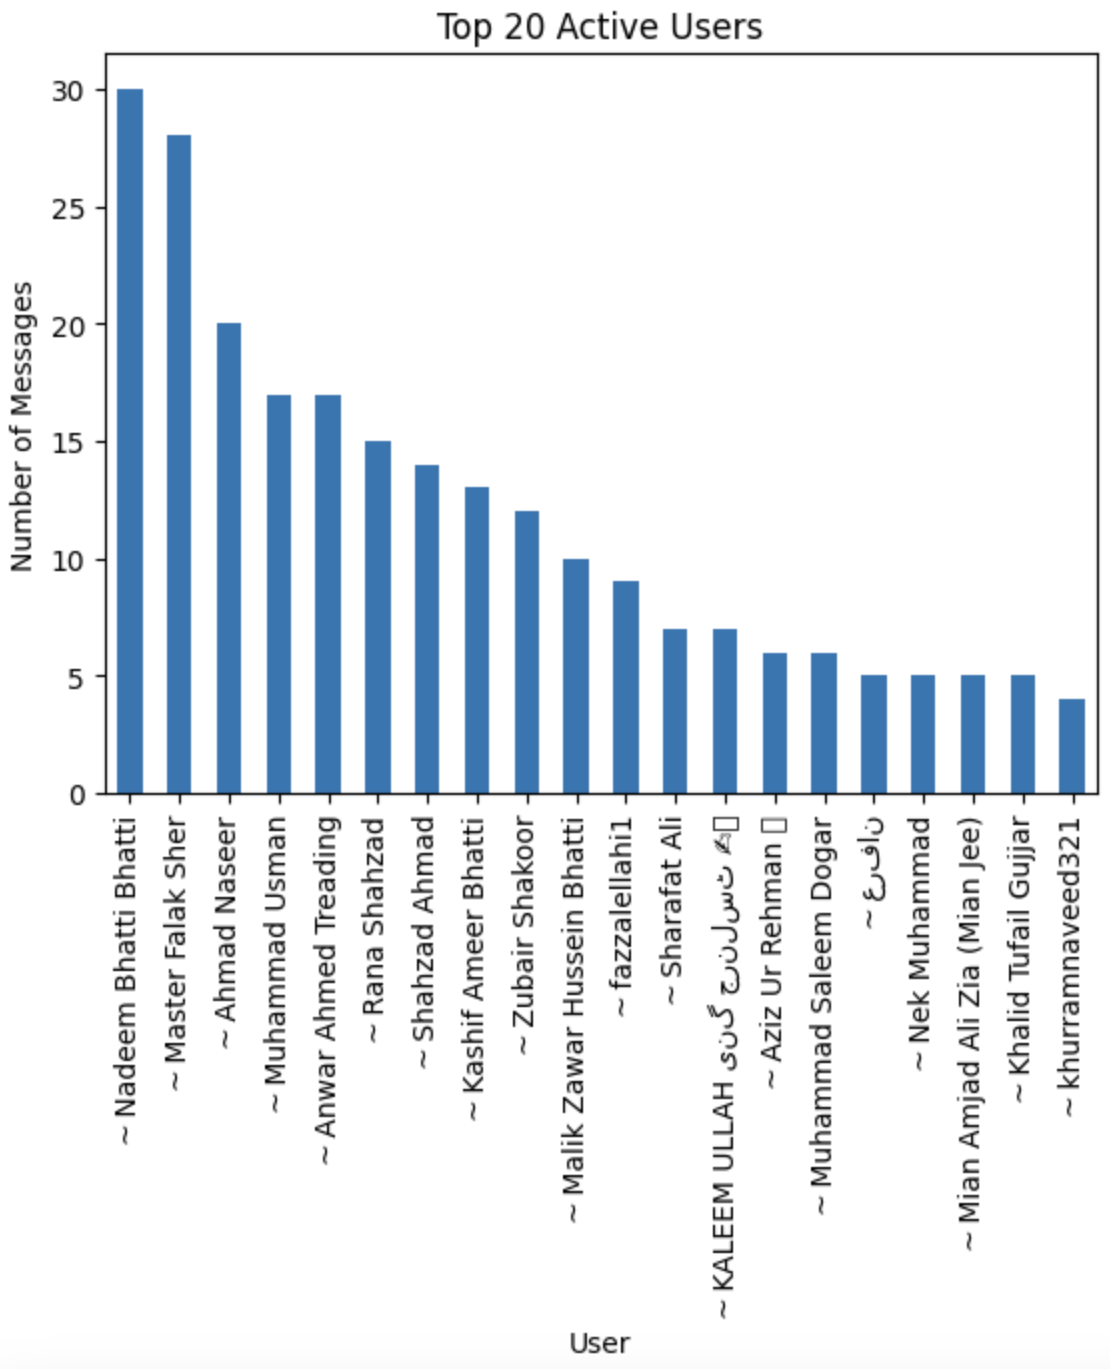
\includegraphics[width=0.8\textwidth]{img/active_users.png}
  \caption{Top 20 Active Users by messages}
\end{figure}

\section{Main Talking Points}
The main talking points in the group are:
\begin{itemize}
    \item Agriculture and Farming Techniques
    \item Weather Updates
    \item Pesticides and Fertilizers
    \item Crop Varieties
    \item Soil Health and Management
    \item Pest Control
    \item Planting Guides
    \item Production Plans
\end{itemize}

\section{Time of Posting}
The most active posting times are 1-2 PM and 5-6 PM, as shown in the chart below.
\begin{figure}[H]
\centering
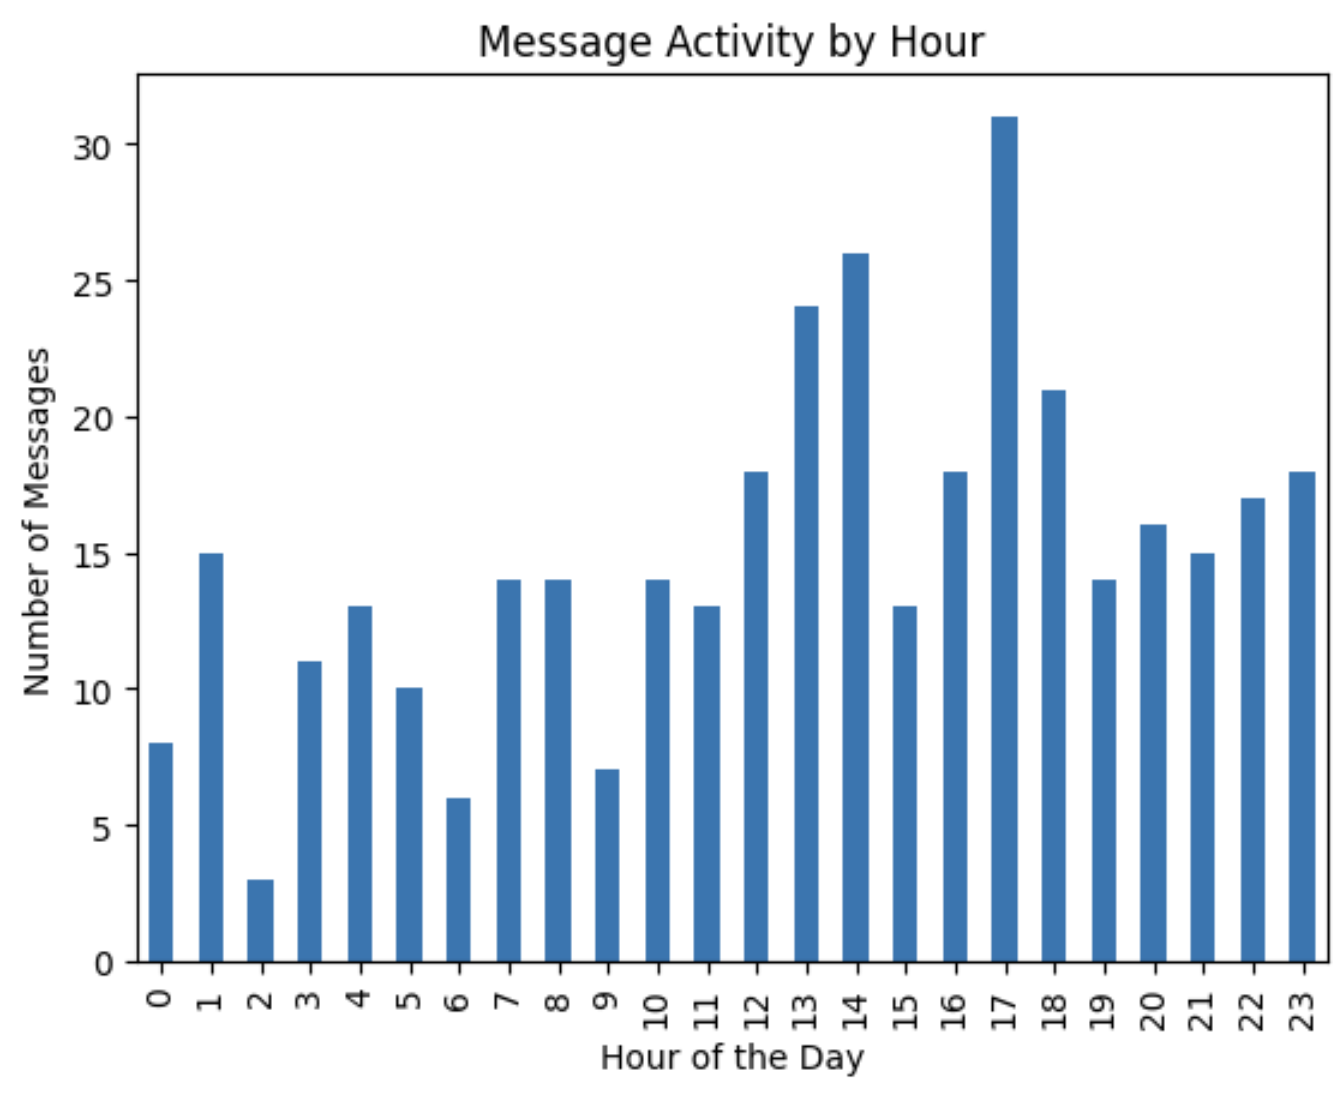
\includegraphics[width=0.8\textwidth]{img/posting_times.png}
\caption{Message Activity by Hour}
\end{figure}

\section{Preferred Medium of Posting}
Text and photos are the most preferred mediums for posting in the group, as shown in the chart below.
\begin{figure}[H]
\centering
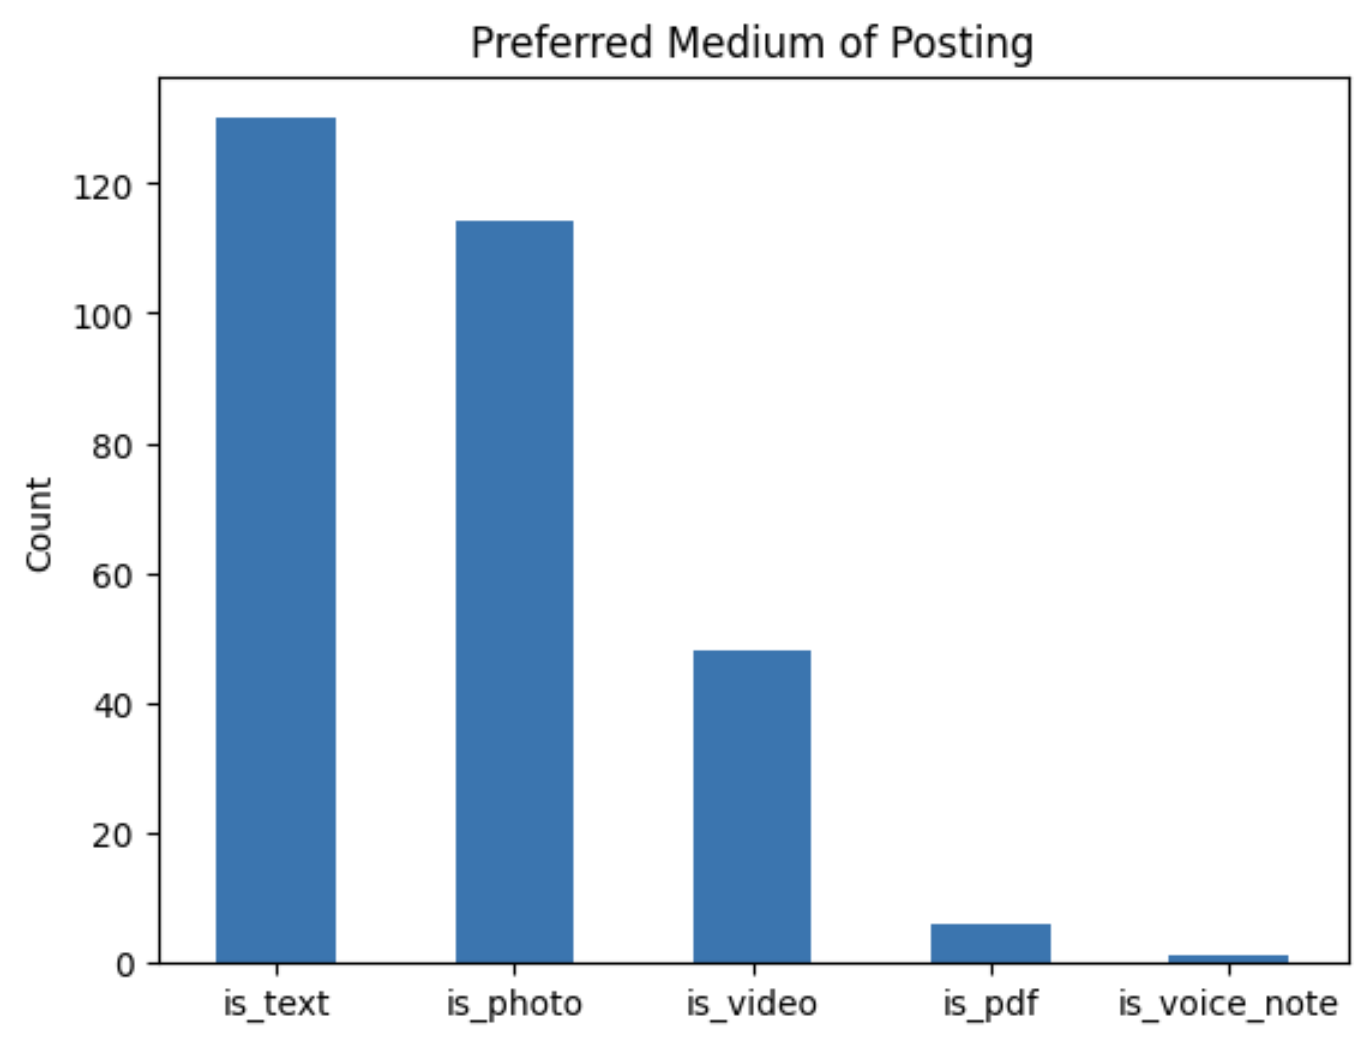
\includegraphics[width=0.8\textwidth]{img/medium_preference.png}
\caption{Preferred Mediums of Posting}
\end{figure}

\section{Conclusion}
The WhatsApp group ``Kissan Express" serves as a platform for sharing agricultural knowledge, techniques, and products among its members. While the group contains a diverse range of content, including marketing posts, religious messages, and political discussions, the primary focus remains on agriculture and farming-related topics. The group's active users engage with each other through text messages, photos, and videos, sharing valuable insights and information to support the agricultural community. By analyzing the group's content, user interactions, and posting patterns, this report provides a comprehensive overview of the group's dynamics and main talking points, highlighting the importance of agriculture in the group's communication.

\end{document}
